\chapter{Sequential Monte Carlo for Bayesian Model Comparison}
\label{cha:Sequential Monte Carlo for Bayesian Model Comparison}

As reviewed in chapter~\ref{cha:Monte Carlo Methods}, \mcmc algorithms, though
widely used for the purpose of Bayesian computation, have many limitations.
Algorithms such as \rjmcmc are conceptually appealing, yet often difficult to
design in practice. Other algorithms such as the Metropolis-Hastings
algorithm, though provides a generic framework which can be applied in many
fields, the design of efficient, high performance algorithms still requires
considerable expertise and sometimes extensive experience.

In recent years, there is a tendency of considering population based
algorithms.  A common theme in these algorithms is that, instead of simulating
directly from complex target distribution, related yet simpler distributions
are used to ``help'' the simulation. One of such algorithm, which is
essentially a generalization of the Metropolis-Hastings algorithm, population
\mcmc is reviewed in section~\ref{sub:Population mcmc}, in which the easier to
simulate distribution ``lends'' information to the target and fastens its
mixing.  Another example of population based algorithm is the recent
development of particular \mcmc \cite{Andrieu:2010gc}, which embed \smc
samplers, which will be the central topic of this chapter, inside \mcmc
algorithms.

Sequential Monte Carlo (\smc) samplers, in various forms has been around for
more than a decade and widely used in many fields. Until recent there is
little interest of using it for Bayesian model comparison for a few reasons.
One of the more important one is that, when \mcmc algorithms are available,
\smc could cost more computational resources than a well designed \mcmc
algorithm. However we believe there are at least two important reasons that
\smc can be preferable to \mcmc for the purpose of Bayesian model comparison.

First, it provides a generic and robust framework for simulation from complex
distributions that are previously difficult for \mcmc algorithms, especially
for high dimensional multinode distributions. Though it is not impossible to
design \mcmc algorithms for the same problems, it can be hugely difficult in
practice. The \smc framework provides a vital alternative that is easy to use.
It has the potential to enable statisticians to construct more realistic,
useful models that were previously difficult, if not impossible, to use due to
the computational complexity. Second, most Monte Carlo algorithms has to be
implemented on computers to be useful. Therefore it is unrealistic to not
consider the trend of today's computer technologies. Parallel computing has
become commodity in recent years. And \smc is much more suitable for this kind
of computing than conventional \mcmc. There are many attempts of parallelizing
\mcmc algorithms. However, as we will see later, \smc has certain advantage
over some of them.

In this chapter, we first give a review of \smc algorithms in
section~\ref{sec:Sequential Monte Carlo samplers}. It is followed by a section
details the use of \smc in the context of Bayesian model comparison. Next,
section~\ref{sec:Extensions and refinements} develops some extensions and
refinements of existing practices. Last, we conclude this chapter with a
discussion of how the presented framework lead to an automatic and generic
algorithms.

The application of \smc samplers to the Bayesian model comparison problem is
straightforward. However, it has been overlooked in recent years. In this
section, we outline common strategies of using \smc samplers for Bayesian
model comparison. In the next section, we introduce some innovative refinement
and extensions to existing practices. As consistent with this thesis, the \pet
compartmental model will be used as a running example to illustrate various
methodologies. We will consider both simulated and real world data. The
simulated data set is the same as in chapter~\ref{cha:Introduction}. Due to
the large amount of the real data, it is beyond the resources we have to
perform repeated simulations for a whole \pet scan. Instead, 20 real data sets
are sampled from typical region of interest in a single \pet scan.
Figure~\ref{fig:typical real pet} shows three of them. As we can see, they
varies considerably in characteristics despite all can be described as
``typical'' \pet data. The purpose of the current work is to advocate robust
and self-tuning algorithms. And the variability in the data sets provides
excellent test examples. In addition, in this chapter, the models are
configured with the non-informative priors and thus the parameters are
exchangeable, similar to that of a mixture model. This creates a multimodal
posterior surface for models with two or more components.

\begin{figure}
  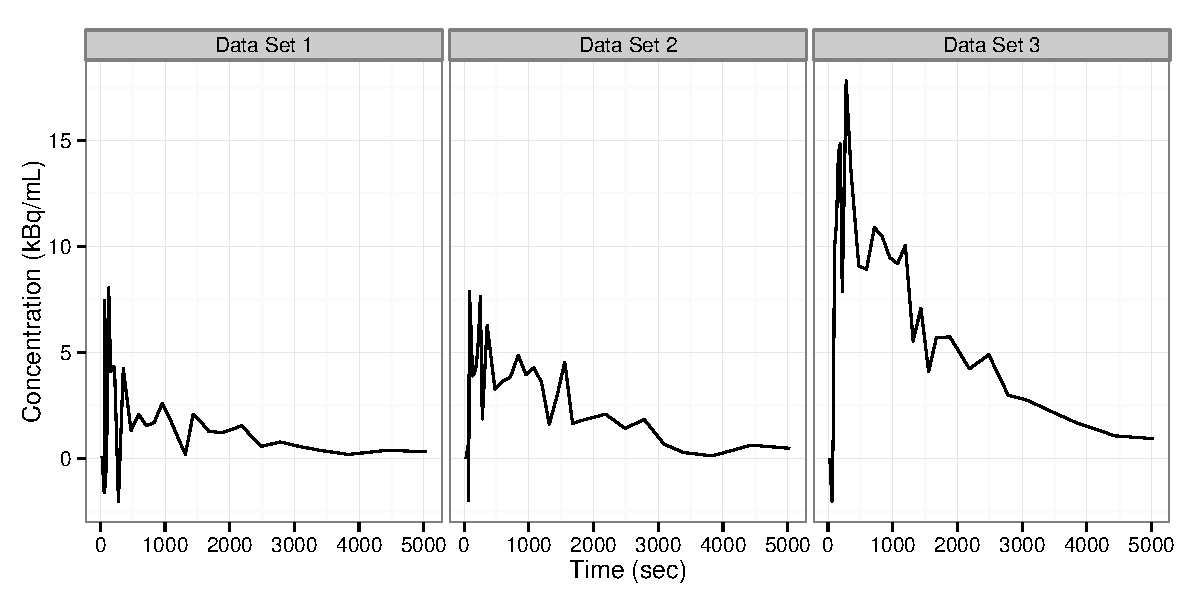
\includegraphics[width=\linewidth]{fig/Typical_PET}
  \caption{Typical real \pet data}
\end{figure}

\section{Sequential Monte Carlo samplers}
\label{sec:Sequential Monte Carlo samplers}

\smc samplers allow us to obtain, iteratively, collections of weighted samples
from a sequence of distribution $\{\pi_t\}_{t\ge0}$ over essentially any
random variables on some measurable spaces $(E_t,\calE_t)$. It is an extension
of the \emph{sequential importance sampling} (\sis) techniques. It is a
generalization of particle filter algorithms widely used in physics and signal
tracking literature. In the remaining of this section, the sequential
importance sampling and resampling algorithms are introduced. Then how they
are generalized to \smc samplers for the purpose of the current work are
discussed.

\subsection{Sequential importance sampling and resampling}
\label{sub:Sequential importance sampling and resampling}

Sequential importance sampling (\sis) generalizes the importance sampling (see
section~\ref{sec:Classical Monte Carlo and importance sampling}) technique for
a sequence of distributions $\{\pi_t\}_{t\ge0}$ defined on spaces
$\{\prod_{k=0}^tE_k\}_{t\ge0}$. At time $t = 0$, sample
$\{X_0^{(i)}\}_{i=1}^N$ from $\eta_0$ and compute the weights $W_0^{(i)}
\propto \pi_0(X_0^{(i)})/\eta_0(X_0^{(i)})$. At time $t\ge1$, each sample
$X_{0:t-1}^{(i)}$, usually termed \emph{particles} in the literature, is
extended to $X_{0:t}^{(i)}$ by a proposal distribution
$q_t(\cdot|X_{0:t-1}^{(i)})$. And the weights are recalculated by $W_t^{(i)}
\propto \pi_t(X_{0:t}^{(i)})/\eta_t(X_{0:t}^{(i)})$ where
\begin{equation}
  \eta_t(X_{0:t}^{(i)}) =
  \eta_{t-1}(X_{0:t-1}^{(i)})q_t(X_{0:t}^{(i)}|X_{0:t-1}^{(i)})
\end{equation}
and thus
\begin{align}
  W_t^{(i)} \propto \frac{\pi_t(X_{0:t}^{(i)})}{\eta_t(X_{0:t}^{(i)})}
  &= \frac{\pi_t(X_{0:t}^{(i)})\pi_{t-1}(X_{0:t-1}^{(i)})}
  {\eta_{t-1}(X_{0:t-1}^{(i)})q_t(X_{0:t}^{(i)}|X_{0:t-1}^{(i)})
    \pi_{t-1}(X_{0:t-1}^{(i)})} \notag\\
  &= \frac{\pi_t(X_{0:t}^{(i)})}
  {q_t(X_{0:t}^{(i)}|X_{0:t-1}^{(i)})\pi_{t-1}(X_{0:t-1}^{(i)})}W_{t-1}^{(i)}
  \label{eq:si}
\end{align}
and importance sampling estimate of $\Exp_{\pi_t}[\varphi_t(X_{0:t})]$ can be
obtained using $\{W_t^{(i)},X_{0:t}^{(i)}\}_{i=1}^N$.

However this approach fails as $t$ becomes large. The weights tend to become
concentrated on a few particles as the discrepancy between $\eta_t$ and
$\pi_t$ becomes larger. Resampling techniques are applied such that, a new
particle system $\{\bar{W}_t^{(i)},\bar{X}_{0:t}^{(i)}\}_{i=1}^M$ is obtained
with the property,
\begin{equation}
  \Exp\Bigl[\sum_{i=1}^M\bar{W}_t^{(i)}\varphi_t(\bar{X}_{0:t}^{(i)})\Bigr] =
  \Exp\Bigl[\sum_{i=1}^NW_t^{(i)}\varphi_t(X_{0:t}^{(i)})\Bigr]
  \label{eq:resample}
\end{equation}
In practice, the resampling algorithm is usually chosen such that $M = N$ and
$\bar{W}^{(i)} = 1/N$ for $i=1,\dots,N$. Resampling can be performed at each time
$t$ or adaptively based on some criteria of the discrepancy. One popular
quantity used to monitor the discrepancy is \emph{effective sample size}
(\ess), introduced by \cite{Liu:1998iu}, defined as
\begin{equation}
  \ess_t = \frac{1}{\sum_{i=1}^N (W_t^{(i)})^2}
\end{equation}
where $\{W_t^{(i)}\}_{i=1}^N$ are the normalized weights. And resampling can
be performed when $\ess\le \alpha N$ where $\alpha\in[0,1]$.

The common practice of resampling is to replicate particles with large weights
and discard those with small weights. In other words, instead of generating a
random sample $\{\bar{X}_{0:t}^{(i)}\}_{i=1}^N$ directly, a random sample of
integers $\{R^{(i)}\}_{i=1}^N$ is generated, such that $R^{(i)} \ge 0$ for $i
= 1,\dots,N$ and $\sum_{i=1}^N R^{(i)} = N$. And each particle value
$X_{0:t}^{(i)}$ is replicated for $R^{(i)}$ times in the new particle system.
The distribution of $\{R^{(i)}\}_{i=1}^N$ shall fulfill the requirement of
Equation~\ref{eq:resample}. One such distribution is a multinomial
distribution of size $N$ and weights $(W_t^{(i)},\dots,W_t^{(N)})$. See
\cite{Douc:2005wa} for some commonly used resampling algorithms.

\subsection[SMC samplers]{\protect\smc samplers}
\label{sub:SMC Samplers}

\smc samplers allow us to obtain, iteratively, collections of weighted samples
from a sequence of distributions $\{\pi_t\}_{t\ge0}$ over essentially any
random variables on some spaces $\{E_t\}_{t\ge0}$, by constructing a sequence
of auxiliary distributions $\{\tilde\pi_t\}_{t\ge0}$ on spaces of increasing
dimensions, $\tilde\pi_t(x_{0:t})=\pi_t (x_t) \prod_{s=0}^{t-1}
L_s(x_{s+1},x_s)$, where the sequence of Markov kernels $\{L_s\}_{s=0}^{t-1}$,
termed backward kernels, is formally arbitrary but critically influences the
estimator variance. See \cite{DelMoral:2006hc} for further details and
guidance on the selection of these kernels.

Standard sequential importance sampling and resampling algorithms can then be
applied to the sequence of synthetic distributions, $\{\tilde\pi_t\}_{t\ge0}$.
At time $t - 1$, assume that a set of weighted particles
$\{W_{t-1}^{(i)},X_{0:t-1}^{(i)}\}_{i=1}^N$ approximating $\tilde\pi_{t-1}$ is
available, then at time $t$, the path of each particle is extended with a
Markov kernel say, $K_t(x_{t-1}, x_t)$ and the set of particles
$\{X_{0:t}^{(i)}\}_{i=1}^N$ reach the distribution $\eta_t(X_{0:t}^{(i)}) =
\eta_0(X_0^{(i)})\prod_{k=1}^tK_t(X_{t-1}^{(i)}, X_t^{(i)})$, where $\eta_0$
is the initial distribution of the particles. To correct the discrepancy
between $\eta_t$ and $\tilde\pi_t$, Equation~\ref{eq:si} is applied and in
this case,
\begin{equation}
  W_t^{(i)} \propto \frac{\tilde\pi_t(X_{0:t}^{(i)})}{\eta_t(X_{0:t}^{(i)})}
  = \frac{\pi_t(X_t^{(i)})\prod_{s=0}^{t-1}L_s(X_{s+1}^{(i)}, X_s^{(i)})}
  {\eta_0(X_0^{(i)})\prod_{k=1}^tK_t(X_{t-1}^{(i)},X_t^{(i)})}
  \propto \tilde{w}_t(X_{t-1}^{(i)}, X_t^{(i)})W_{t-1}^{(i)}
\end{equation}
where $\tilde{w}_t$, termed the \emph{incremental weights}, are calculated as,
\begin{equation}
  \tilde{w}_t(X_{t-1}^{(i)},X_t^{(i)}) =
  \frac{\pi_t(X_t^{(i)})L_{t-1}(X_t^{(i)}, X_{t-1}^{(i)})}
  {\pi_{t-1}(X_{t-1}^{(i)})K_t(X_{t-1}^{(i)}, X_t^{(i)})}
\end{equation}
If $\pi_t$ is only known up to a normalizing constant, say $\pi_t(x_t) =
\gamma_t(x_t)/Z_t$, then we can use the \emph{unnormalized} incremental
weights
\begin{equation}
  w_t(X_{t-1}^{(i)},X_t^{(i)}) =
  \frac{\gamma_t(X_t^{(i)})L_{t-1}(X_t^{(i)}, X_{t-1}^{(i)})}
  {\gamma_{t-1}(X_{t-1}^{(i)})K_t(X_{t-1}^{(i)}, X_t^{(i)})}
\end{equation}
for importance sampling. Further, with the previously \emph{normalized}
weights $\{W_{t-1}^{(i)}\}_{i=1}^N$, we can estimate the ratio of normalizing
constant $Z_t/Z_{t-1}$ by
\begin{equation}
  \frac{\hat{Z}_t}{Z_{t-1}} =
  \sum_{i=1}^N W_{t-1}^{(i)}w_t(X_{t-1}^{(i)},X_t^{(i)})
\end{equation}
Sequentially, the normalizing constant between initial distribution $\pi_0$
and some target $\pi_T$, $T\ge1$ can be estimated. See \cite{DelMoral:2006hc}
for details on calculating the incremental weights. In practice, when $K_t$ is
invariant to $\pi_t$, and an approximated suboptimal backward kernel
\begin{equation}
  L_{t-1}(x_t, x_{t-1}) = \frac{\pi(x_{t-1})K_t(x_{t-1}, x_t)}{\pi_t(x_t)}
\end{equation}
is used, the unnormalized incremental weights will be
\begin{equation}
  w_t(X_{t-1}^{(i)},X_t^{(i)}) =
  \frac{\gamma_t(X_{t-1}^{(i)})}{\gamma_{t-1}(X_{t-1}^{(i)})}.
  \label{eq:inc_weight_mcmc}
\end{equation}

\section{Application to Bayesian model comparison}
\label{sec:Application to Bayesian model comparison}

The problem of interest is characterizing the posterior distribution over
$\{\Mk\}_{k\in\calK}$, a set of possible models, with model $\Mk$ having
parameter vector $\paramk\in\Paramk$ which must also usually be inferred.
Given prior distributions $\pi(\Mk)$ and $\pi(\paramk|\Mk)$ and likelihood
$p(\data|\paramk,\Mk)$ we seek the posterior distributions $\pi(\Mk|\data)
\propto p(\data|\Mk)$. There are three fundamentally different approaches to
the computations,
\begin{enumerate}
  \item Calculate posterior model probabilities directly.
  \item Calculate the evidence, $p(\data|\Mk)$, of each model.
  \item Calculate pairwise evidence ratios.
\end{enumerate}
Each approach admits a natural \smc strategy.

\subsection{\smc1: An all-in-one approach}
\label{sub:smc1: An all-in-one approach}

One could consider obtaining samples from the same distribution employed in
the \rjmcmc approach to model comparison, namely:
\begin{equation}
  \pi^{(1)}(\Mk,\paramk) \propto \pi(\Mk)\pi(\paramk|\Mk)p(\data|\paramk,\Mk)
\end{equation}
which is defined on the disjoint union space
$\bigcup_{k\in\calK}(\{\Mk\}\times\Paramk)$.

One obvious \smc approach is to define a sequence of distributions
$\{\pi_t^{(1)}\}_{t=0}^T$ such that $\pi^{(1)}_0$ is easy to sample from,
$\pi_{T}^{(1)} = \pi^{(1)}$ and the intermediate distributions move smoothly
between them. In the remainder of this section, we use the notation
$(\Mk[t],\paramk[t])$ to denote a random sample on the space
$\bigcup_{k\in\calK}(\{\Mk\}\times\Paramk)$ at time $t$. One simple approach,
which might be expected to work well, is the use of an annealing scheme such
that:
\begin{equation}
  \pi^{(1)}_t(\Mk[t],\paramk[t]) \propto \pi(\Mk[t])\pi(\paramk[t]|\Mk[t])
  p(\data|\paramk[t],\Mk[t])^{\alpha(t/T)},
  \label{eq:geometry_1}
\end{equation}
for some monotonically increasing $\alpha:[0,1]\to[0,1]$ such that $\alpha(0)
= 0$ and $\alpha(1) = 1$. Other approaches are possible and might prove more
efficient for some problems (such as the ``data tempering'' approach which
\cite{Chopin:2002hg} proposed for parameter estimation which could easily
be incorporated in our framework), but this strategy provides a convenient
generic approach. These choices lead to Algorithm~\ref{alg:smc1}.

% $\alpha$ provides an \emph{annealing schedule} which is intended to allow
% the control of the discrepancy between pairs of adjacent distributions. This
% gives the joint prior on model order and parameters as an initial
% distribution and gradually introduces the influence of the likelihood until
% the full posterior is reached.

% Given a weighted collection of samples $\{W^{(k,i)}_T, X^{(k,i)}_{T} =
% (K_T^{(k,i)},\theta_T^{(k,i)})\}_{i=1}^N$ targeting $\pi^{(1)}$, one may
% approximate the two distributions of interest using the empirical measures:
% \begin{align*}
%   \widehat{\pi}^{(1)}(K = k) &= \sum\limits_{i=1}^N W^{(k,i)} \delta_{k,
%   K^{(k,i)}_T} \\
%   \widehat{\pi}^{(1)}(d\theta|K=k) &= \frac{1}{\widehat{\pi}^{(1)}(K = k)}
%   \sum\limits_{i=1}^N W^{(k,i)} \delta_{k, K_T^{(k,i)}}
%   \delta_{\theta^{(k,i)}_T}(d\theta),
% \end{align*}
% where $\delta_{k,K^{(k,i)}_T}$ denotes the \emph{Kronecker} delta and
% $\delta_{\theta{(k,i)}}$ denotes the Dirac measure concentrated at
% $\theta^{(k,i)}$.

% Thus, the output of such an \smc algorithm may be used as a (weighted)
% equivalent to that from a suitable \rjmcmc algorithm, with the posterior
% probability of each model corresponding to the (weighted) proportion of
% samples from that model.

This approach might outperform \rjmcmc when it is difficult to design
fast-mixing Markov kernels. There are many examples of such an annealed \smc
strategy outperforming \mcmc at a given computational cost --- see, for
example, \cite{Fan:2008tf,Johansen:2008kp,Fearnhead:2010ua}. Such
trans-dimensional \smc has been proposed in several contexts
\cite{Peters:2005wh} and an extension proposed and analysed
by \cite{Jasra:2008bb}.

\begin{algorithm}
\begin{algorithmic}
  \STATE \emph{Initialisation:} Set $t\leftarrow0$.
  \STATE\STATESKIP Sample $X_0^{(i)} = (M_0^{(i)},\theta_0^{(i)})\sim\nu$
  for some proposal distribution $\nu$ (usually the joint prior).
  \STATE\STATESKIP Weight $W_0^{(i)} \propto w_0(X_0^{(i)}) =
  {\pi(M_0^{(i)}) \pi(\theta^{(i)}_0|M_0^{(i)})}/
  {\nu(M_0^{(i)},\theta_0^{(i)})}$.
  \STATE\STATESKIP Apply resampling if necessary (e.g., if \ess
  \cite{Kong:1994ul} less than some threshold).

  \STATE \emph{Iteration:} Set $t\leftarrow t + 1$.
  \STATE\STATESKIP Weight $W_t^{(i)} \propto W_{t-1}^{(i)}
  p(\data|\theta_{t-1}^{(i)},M_{t-1}^{(i)})^{\alpha(t/T) - \alpha([t-1]/T)}$.
  \STATE\STATESKIP Apply resampling if necessary.
  \STATE\STATESKIP Sample $X_t^{(i)} \sim K_t(\cdot|X_{t-1}^{(i)})$, a
  $\pi_t^{(1)}$-invariant kernel.

  \STATE \emph{Repeat} the \emph{Iteration} step \emph{until $t = T$}.
\end{algorithmic}
\caption{\smc1: An All-in-One Approach to Model Comparison.}\label{alg:smc1}
\end{algorithm}

We include this approach for completeness and study it empirically later.
However, the more direct approaches described in the following sections lead
more naturally to easy-to-implement strategies with good performance.

\subsection{\smc2: A direct-evidence-calculation approach}
\label{sub:smc2: A direct-evidence-calculation approach}

An alternative approach would be to estimate explicitly the evidence
associated with each model. We propose to do this by sampling from a sequence
of distributions for each model: starting from the parameter prior and
sweeping through a sequence of distributions to the posterior.

Numerous strategies are possible to construct such a sequence of
distributions, but one option is to use for each model $\Mk$, $k\in\calK$, the
sequence $\{\pi_t^{(2,k)}\}_{t=0}^{T_k}$, defined by
\begin{equation}
  \pi_t^{(2,k)}(\paramk[t]) \propto
  \pi(\paramk[t]|\Mk)p(\data|\paramk[t],\Mk)^{\alpha_k(t/T_k)}.
  \label{eq:geometry_2}
\end{equation}
where the number of distribution $T_k$, and the annealing schedule,
$\alpha_k:[0,1]\to[0,1]$ may be different for each model. This leads to
Algorithm~\ref{alg:smc2}.

The estimator of the posterior model probabilities depends upon the approach
taken to estimate the normalizing constant. Direct estimation of the evidence
can be performed using the output of this \smc algorithm and the standard
unbiased estimator, termed \smc2-\ds below:
\begin{equation}\label{eq:smc2-ds}
  \sum_{i=1}^N \frac{\pi(\theta_0^{(k,i)}|\Mk)}{\nu(\theta_0^{(k,i)})} \times
  \prod_{t=2}^T \sum_{i=1}^N W_{t-1}^{(k,i)}
  p(\data|\theta_{t-1}^{(k,i)}\Mk)^{\alpha_k(t/T_k) - \alpha_k([t-1]/T_k)}
\end{equation}
where $W_{t-1}^{(k,i)}$ is the importance weight of sample $i$,
$\theta_{t-1}^{(k,i)}$, during iteration $t-1$ for model $\Mk$. An alternative
approach to computing the evidence is also worthy of consideration. As has
been suggested, and shown to perform well empirically previously \cite[see,
for example]{Johansen:2006wm}, it is possible to use all of the samples from
every generation of an \smc sampler to approximate the path sampling estimator
and hence to obtain an estimate of the ratio of normalizing constants.
Section~\ref{sub:Path Sampling via smc2/smc3} provides details.

The posterior distribution of the parameters conditional upon a particular
model can also be approximated with:
\begin{equation*}
  \widehat{\pi}_{T_k}^{(2,k)}(\diff\theta) =
  \sum\limits_{i=1}^{N} W_{T_k}^{(k,i)}
  \delta_{\theta^{(k,i)}_{T_k}}(\diff\theta).
\end{equation*}
where $\delta_{\theta^{(k,i)}_{T_k}}$ is the Dirac measure.

% It is straightforward to use different numbers of samples, $N$, for each
% model when appropriate. in settings in which some models can be
% characterised substantially more easily than others.

This approach is appealing for several reasons. One is that it is designed to
estimate directly the quantity of interest: the evidence, producing a sample
from that distribution at the same time. Another advantage of this approach
over \smc1 and the \rjmcmc approach is that it provides as good a
characterisation of each model as is required: it is possible to obtain a good
estimate of the parameters of every model, even those for which the posterior
probability is small. Perhaps most significant is the fact that this approach
does not require the design of proposal distributions or Markov kernels which
move from one model to another: each model is dealt with in isolation. Whilst
this may not be desirable in every situation, there are circumstances in which
efficient moves between models are almost impossible to devise.

This approach also has some disadvantages. In particular, it is necessary to
run a separate simulation for each model --- rendering it impossible to deal
with countable collections of models (although this is not such a substantial
problem in many interesting cases). The ease of implementation may often
offset this limitation.

\begin{algorithm}
\begin{algorithmic}
  \STATE For each model $k \in \calK$ perform the following algorithm.

  \STATE \emph{Initialisation:} Set $t\leftarrow0$.
  \STATE\STATESKIP Sample $\theta_0^{(k,i)}\sim\nu_k$ for some proposal
  distribution $\nu_k$ (usually the parameter prior).
  \STATE\STATESKIP Weight $W_0^{(k,i)} \propto w_0(\theta_0^{(k,i)}) =
  {\pi(\theta_0^{(k,i)}|\Mk)}/{\nu_k(\theta_0^{(k,i)})}$.
  \STATE\STATESKIP Apply resampling if necessary.

  \STATE \emph{Iteration:} Set $t\leftarrow t + 1$.
  \STATE\STATESKIP Weight $W_t^{(k,i)} \propto W_{t-1}^{(k,i)}
  p(\data|\theta_{t-1}^{(k,i)},\Mk)^{\alpha(t/T_k) - \alpha([t-1]/T_k)}$.
  \STATE\STATESKIP Apply resampling if necessary.
  \STATE\STATESKIP Sample $\theta_t^{(k,i)} \sim
  K_t(\cdot|\theta_{t-1}^{(k,i)})$, a $\pi_t^{(k,2)}$-invariant kernel.

  \STATE \emph{Repeat} the \emph{Iteration} step \emph{until $t = T_k$}.
\end{algorithmic}
\caption{\smc2: A Direct-Evidence-Calculation Approach.}\label{alg:smc2}
\end{algorithm}

\subsection{\smc3: A relative-evidence-calculation approach}
\label{sub:smc3: A relative-evidence-calculation approach}

A final approach can be thought of as \emph{sequential model comparison}.
Rather than estimating the evidence associated with any particular model, we
could estimate pairwise evidence ratios directly. The \smc sampler starts with
a initial distribution being the posterior of one model (which could comes
from a separate \smc sampler starting from its prior) and moves towards the
posterior of another related model. Then the sampler can continue towards
another related model.

Given a finite collection of models $\{\Mk\}$, $k\in\calK$, suppose the models
are ordered in a sensible way (e.g., $\Mk[k-1]$ is nested within $\Mk$ or
$\paramk$ is of higher dimension than $\paramk[k-1]$). For each
$k\in\calK$, we consider a sequence of distributions
$\{\pi_t^{(3,k)}\}_{t=0}^{T_k}$, such that $\pi_0^{(3,k)}(\Mk[],\paramk[]) =
\pi(\paramk[]|\data,\Mk) \mathbb{I}_{\{\Mk\}}(\Mk[])$ and $\pi_{T_k}^{(3,k)}(\Mk[],\paramk[]) =
\pi(\paramk[]|\data,\Mk[k+1]) \mathbb{I}_{\{\Mk[k+1]\}}(\Mk[]) = \pi_{0}^{(3,k+1)}(\Mk[],\paramk[])$.
When it is possible to construct a \smc sampler that iterates over this
sequence of distributions, the estimate of the ratio of normalizing constants
is the Bayes factor estimate of model $\Mk[k+1]$ in favour of model $\Mk$.

This approach is conceptually appealing, but requires the construction of a
smooth path between the posterior distributions of interest. The geometric
annealing strategy which has been advocated as a good generic strategy in the
previous sections is only appropriate when the support of successive
distributions is non-increasing. This is unlikely to be the case in
interesting model comparison problems.

In this paper we consider a sequence of distributions on the disjoint union
$\{\Mk,\Paramk\}\cup\{\Mk[k+1],\Paramk[k+1]\},$ with the sequence of
distributions $\{\pi_t^{(3,k)}\}_{t=0}^{T_k}$ defined as the full posterior,
\begin{equation}
  \pi_t^{(3,k)}(\Mk[t],\paramk[t]) \propto
  \pi_t(\Mk[t]) \pi(\paramk[t]|\Mk[t]) p(\data|\paramk[t],\Mk[t])
\end{equation}
where $\Mk[t]\in\{\Mk,\Mk[k+1]\}$ and the prior of models at time $t$,
$\pi_t(\Mk[t])$ is defined by
\begin{equation}
  \pi_t(\Mk[k+1]) = \alpha(t/T_k)
  \label{eq:smc3_prior}
\end{equation}
for some monotonically increasing $\alpha:[0,1]\to[0,1]$ such that $\alpha(0)
= 0$ and $\alpha(1) = 1$. It is clear that the \mcmc moves between iterations
need to be similar to those in the \rjmcmc or \smc1 algorithms. The
difference is that instead of efficient exploration of the whole model space,
only moves between two models are required and the sequence of distributions
employed helps to ensure exploration of both model spaces. The algorithm for
this particular sequence of distribution is outlined in
Algorithm~\ref{alg:smc3}. It can be extended to other possible sequence of
distributions between models.

An advantage of this approach is that it provides direct estimate of the Bayes
factor which is of interest for model comparison purpose while not requiring
exploration of as complicated a space as that employed within \rjmcmc or
\smc1. The estimating of normalizing constant in \smc3 can follows in
exactly the same manner as in the \smc2 case. In \smc3, the same
estimator provides a direct estimate of the Bayes factor.

%Note that the standard \smc unbiased estimator is in fact the
%ratio of normalizing constants between the initial distribution and the final
%distribution. In \smc2, we initialised the system with the prior
%distribution and thus the estimates are directly the evidence for each model.


\begin{algorithm}
\begin{algorithmic}
  \STATE \emph{Initialisation:} Set $k\leftarrow1$.
  \STATE\STATESKIP Use Algorithm~\ref{alg:smc2} to obtain weighted samples
  for $\pi_{T_1}^{(3,1)}$, the parameter posterior for model $\Mk[1]$

  \STATE \emph{Relative Evidence Calculation}
  \STATE\STATESKIP Set $k\leftarrow k + 1$, $t\leftarrow0$.
  \STATE\STATESKIP Denote current weighted samples as
  $\{W_0^{(k,i)},X_0^{(k,i)}\}_{i=1}^N$ where $X_0^{(k,i)} =
  (M_0^{(k,i)},\theta_0^{(k,i)})$
  \STATE\STATESKIP Apply resampling if necessary.

  \STATE\STATESKIP \emph{Iteration:} Set $t\leftarrow t + 1$.
  \STATE\STATESKIP\STATESKIP Weight $W_t^{(k,i)} \propto W_{t-1}^{(k,i)}
  {\pi_t(M_{t-1}^{(k,i)})}/{\pi_{t-1}(M_{t-1}^{(k,i)})}$.
  \STATE\STATESKIP\STATESKIP Apply resampling if necessary.
  \STATE\STATESKIP\STATESKIP Sample $(M_t^{(k,i)},\theta_t^{(ki)}) \sim
  K_t(\cdot|M_{t-1}^{(k,i)}\theta_{t-1}^{(k,i)})$, a $\pi_t^{(3,k)}$-invariant
  kernel.

  \STATE\STATESKIP \emph{Repeat the \emph{Iteration} step up to $t = T_k$}.

  \STATE \emph{Repeat} the \emph{Relative Evidence Calculation} step \emph{until
    sequentially all relative evidences are calculated}.
\end{algorithmic}
\caption{\smc3: A Relative-Evidence-Calculation Approach to Model Comparison.}
\label{alg:smc3}
\end{algorithm}

\subsection{Path Sampling via \smc2/\smc3}
\label{sub:Path Sampling via smc2/smc3}

The estimation of the normalizing constant associated with our sequences of
distributions can be achieved by a Monte Carlo approximation to the \emph{path
  sampling} formulation given by \cite{Gelman:1998ei}. This is similar to the
technique for population \mcmc as described in section~\ref{sec:Bayesian
  computation with Markov chain Monte Carlo}. In the context of \smc, this
approach is also very closely related to the use of \ais for the same purpose
\cite{Neal:2001we} but as will be demonstrated below the incorporation of some
other elements of the more general \smc algorithm family can improve
performance at negligible cost. Recall that, given a parameter $\alpha$ which
defines a family of distributions, $\{p_{\alpha} = q_{\alpha} /
Z_\alpha\}_{\alpha \in [0,1]}$ which move smoothly from $p_0 = q_0 / Z_0$ to
$p_1 = q_1 / Z_1$ as $\alpha$ increases from zero to one, one can estimate the
logarithm of the ratio of their normalizing constants via a simple integral
relationship which holds under very mild regularity conditions:
\begin{equation}
  \log\biggl( \frac{Z_1}{Z_0} \biggr) =
  \int_{0}^{1} \Exp_\alpha \biggl[ \rnd{\log q_{\alpha}(\cdot)}{\alpha}
  \biggr] \intd\alpha, \label{eq:path_identity}
\end{equation}
where $\Exp_\alpha$ denotes expectation under $p_\alpha$. Note that the
sequence of distributions in the \smc2 and \smc3 algorithms above, can both be
interpreted as belonging to such a family of distributions, with $\alpha_t =
\alpha(t/T_k)$, where the mapping $\alpha:[0,1]\to[0,1]$ is again monotonic
with $\alpha(0) = 0$ and $\alpha(1) = 1$.

The \smc sampler provides us with a set of weighted samples obtained from a
sequence of distributions suitable for approximating this integral. At each
$t$ we can obtain an estimate of the expectation within the integral for
$\alpha(t/T)$ via the usual importance sampling estimator, and this integral
can then be approximated via numerical integration. Whenever the sequence
of distributions employed by \smc3 has appropriate differentiability it is
also possible to employ path sampling to estimate, directly, the evidence
ratio via this approach applied to the samples generated by that algorithm. In
general, given an increasing sequence $\{\alpha_t\}_{t=0}^T$ where $\alpha_0 =
0$ and $\alpha_T = 1$, a family of distributions
$\{p_{\alpha}\}_{\alpha\in[0,1]}$ as before, and a \smc sampler that iterates
over the sequence of distribution $\{\pi_t = p_{\alpha_t} =
q_{\alpha_t}/Z_{\alpha_t}\}_{t=0}^T$, then with the weighted samples
$\{W_t^{(j)},X_t^{(j)}\}_{j=1}^N$, and $t = 0,\dots,T$, a path sampling
estimator of the ratio of normalizing constants $\Xi_T = \log(Z_1/Z_0)$
can be approximated (using an elementary trapezoidal scheme) by
\begin{equation}
  \widehat\Xi_{T}^{N} = \sum_{t=1}^T
  \frac{1}{2}(\alpha_t - \alpha_{t - 1})(U_t^N + U_{t-1}^N)
  \label{eq:path_est}
\end{equation}
where
\begin{equation}
  U_t^N = \sum_{j=1}^N
  W_t^{(j)} \rnd{\log q_{\alpha}(X_t^{(j)})}{\alpha}\Bigm|_{\alpha = \alpha_t}
\end{equation}

We term these estimators \smc2-\ps and \smc3-\ps in the followings. The
combination of \smc and path sampling is somewhat natural and has been
proposed before, e.g., \cite{Johansen:2006wm} although not there in a Bayesian
context. Despite the good performance observed in the setting of rare
event simulation, the estimation of normalizing constants by this approach
seems to have received little attention in the literature. We suspect that
this is because of widespread acceptance of the suggestion of
\cite{DelMoral:2006hc}, that \smc doesn't outperform \ais when normalizing
constants are the object of inference or that of \cite{Calderhead:2009bd}
that all simulation-based estimators based around path sampling can be
expected to behave similarly. We will demonstrate below that these
observations, whilst true in certain contexts, do not hold in full generality.

\section{Extensions and refinements}
\label{sec:Extensions and refinements}

The algorithms introduced in the last section can be seen as straightforward
application of the well established \smc algorithms to Bayesian model
comparison. Though by construction, \smc algorithms can be more robust than
many \mcmc and other algorithms. However, as with any Monte Carlo algorithms,
without careful design, the performance can be far from satisfactory for many
realistic applications. In this section, we introduce some extensions and
refinement that can further improve the presented framework. Of course, they
cannot guarantee that the algorithms will perform well for all possible
situations. However, it provide robust and reliable solutions for many
realistic applications with minimal manual tuning of the algorithm. Further,
for more difficult problems, they provide a vital foundation on top of which
higher performance algorithms can be built.

\subsection{Improved univariate numerical integration}
\label{sub:Improved univariate numerical integration}

As seen in the last section, the path sampling estimator requires evaluation of
the expectation,
\begin{equation*}
  \Exp_\alpha \biggl[ \rnd{\log q_{\alpha}(\cdot)}{\alpha} \biggr]
\end{equation*}
for $\alpha\in[0,1]$, which can be approximated by importance sampling using
samples generated by a \smc sampler operating on the sequence of distributions
$\{\pi_t = p_{\alpha_t} = q_{\alpha_t}/Z_t\}_{t=0}^T$ directly for
$\alpha\in\{\alpha_t\}_{t=0}^T$. For arbitrary $\alpha\in[0,1]$, finding $t$
such that $\alpha\in(\alpha_{t-1},\alpha_t)$, the expectation can be easily
approximated using existing \smc samples --- the quantities required in the
importance weights to obtain such an estimate have already been calculated
during the running of the \smc algorithm and such computations have little
computational cost. %Indeed, in settings in which the \smc importance weights
%for target distribution $\pi_{\alpha}$ depend only upon the sample at time
%$t-1$, as in the proposed algorithms, the computational cost of the new
%weights are often minimal compared to generate new samples.

As noted by \cite{Friel:2012}  we can use more sophisticated numerical
integration strategies to reduce the path sampling estimator bias. For
example, higher order Newton-Cotes rules rather than the Trapezoidal rule can
be implemented straightforwardly. In the case of SMC it is especially
straightforward to estimate the required expectations at arbitrary $\alpha$
and so we cheaply use higher order integration schemes and we can also use
numerical integrations which make use of a finer mesh
$\{\alpha_t'\}_{t=0}^{T'}$ than $\{\alpha_t\}_{t=0}^T$. Since higher order
numerical integrations based on approximations of derivatives obtained from
Monte Carlo methods may potentially be unstable in some situations, the second
approach can be more appealing in some applications. A demonstration of the
bias reduction effect is provided in Section~\ref{sub:Positron Emission
  Tomography Compartmental Model}.

% It is straightforwardly possible to use more sophisticated numerical
% integration techniques in order to evaluate the approximation of the path
% sampling estimator. Even in the presence of adaptive annealing schemes, it
% is reasonably straightforward to implement higher order schemes than the
% simple Trapezoidal approximation. In a related setting, this was shown to
% provide an appreciable reduction in bias by \cite{Friel:2012}. In our
% context we have found that the bias of even the simple Trapezoidal scheme is
% inconsequential in the regime in which the variance of this method is small
% enough to be competitive and so in the interests of parsimony we have not
% investigated such schemes.

% It is possible to use numerical integration methods other than the
% Trapezoidal rules to improve the path sampling estimator. For example, in a
% \smc2 algorithm, if a sequence of distribution indexed by
% $\{\alpha(t/T)\}_{t=0}^T$ are used, where the path sampling integration is
% with respect to $\alpha\in[0,1]$. Then by placing an additional set of
% distributions at middle points
% $\{(\alpha(t/T)+\alpha((t+1)/T))/2\}_{t=0}^{T-1}$, Simpson's rule can be
% applied and can reduce the bias of the estimator given the same total number
% of distributions in some situations. Using similar techniques, other methods
% of numerical integration an be applied easily as well.

% There may or may not be a significant improvement through using these more
% sophisticated numerical integration methods, as other factors of the sampler
% may dominate the bias and variance of the estimates. Nonetheless, with very
% little effort, this kind of refinement is possible in principal within the
% \smc-\ps framework.

\subsection{Adaptive specification of distributions}
\label{sub:Adaptive specification of distributions}

In settings in which the importance weights at time $t$ depend only upon the
sample at time $t-1$, such as that considered here, it is relatively
straightforward to consider sample-dependent, adapative specification of the
sequence of distributions (typically by choosing the value of a tempering
parameter, such as $\alpha_t$ based upon the current sample).  In
\cite{Jasra:2010eh} such a method of adaptive placing the distributions in
\smc algorithms based on controlling the rate at which the effective sample
size (\ess; \cite{Kong:1994ul}) falls was proposed. With very little
computation cost, this provides an automatic method of specifying a tempering
schedule in such a way that the \ess decays in a regular fashion.
\cite[Algorithm 2]{Schafer:2011bx} used a similar technique but by moving the
particle system only when it resamples they are in a setting which would be
equivalent to resampling at every time step (with longer time steps, followed
by multiple applications of the MCMC kernel) in our formulation. We advocate
resampling only adaptively when \ess is smaller than certain preset threshold,
and here we propose a more general adaptive scheme for the selection of the
sequence of distributions which has significantly better properties when
adaptive resampling is employed.

The \ess was designed to assess the loss of efficiency arising from the use a
simple weighted sample (rather than a simple random sample from the
distribution of interest) in the computation of expectations. It's obtained by
considering a sample approximation of a low order Taylor expansion of the
variance of the importance sampling estimator of an arbitrary test function to
that of the simple Monte Carlo estimator; the test function itself vanishes
from the expression as a consequence of this low order expansion.

In our context, allowing $W_{t-1}^{(i)}$ to denote the \emph{normalized
  weights} of particle $i$ at the end of time $t - 1$, and $w_t^{(i)}$ to
denote the \emph{unnormalized} incremental weights of particle $i$ during
iteration $t$ the \ess calculated using the current weight of each particle is
simply:
\begin{equation}
  \ess_t = \left[ {\sum_{j=1}^N\left( \frac{W_{t-1}^{(j)}
          w_t^{(j)}}{\sum_{k=1}^NW_{t-1}^{(k)}w_t^{(k)}}\right)^2}
  \right]^{-1} = \frac{\bigl(\sum_{j=1}^NW_{t-1}^{(j)}w_t^{(j)}\bigr)^2}
  {\sum_{k=1}^N\bigl(W_{t-1}^{(k)}\bigr)^2\bigl(w_t^{(k)}\bigr)^2}
\end{equation}
It's clearly appropriate to use this quantity (which corresponds to the
coefficient of variation of the current normalized importance weights) to
assess weight degeneracy and to make decisions about appropriate resampling
times (cf. \cite{DelMoral:2012jq}) but it is rather less apparent that it's
the correct quantity to consider when adaptively specifying a sequence of
distributions in an \smc sampler.

The \ess of the current sample weights tells us about the accumulated mismatch
between proposal and target distributions (on an extended space including the
full trajectory of the sample paths) since the last resampling time. Fixing
either the relative or absolute reduction in \ess between successive
distributions does \emph{not} lead to a common discrepancy between successive
distributions unless resampling is conducted after every iteration as will be
demonstrated below.

When specifying a sequence of distributions it is natural to aim for a similar
discrepancy between each pair of successive distributions. In the context of
effective sample size, the natural question to ask is consequently, how large
can we make $\alpha_t - \alpha_{t-1}$ whilst ensuring that $\pi_{t}$ remains
sufficiently similar to $\pi_{t-1}$. One way to measure the discrepancy would
be to consider how good an importance sampling proposal $\pi_{t-1}$ would be
for the estimation of expectations under $\pi_t$ and a natural way to measure
this is via the sample approximation of a Taylor expansion of the relative
variance of such an estimator exactly as in the \ess.

Such a procedure leads us to a quantity which we have termed the
\emph{conditional} \ess (\cess):
\begin{equation}
  \cess_t = \left[ {\sum_{j=1}^N N W_{t-1}^{(j)} \left(
        \frac{w_t^{(j)}}{\sum_{k=1}^N
          N W_{t-1}^{(k)}w_t^{(k)}}\right)^2} \right]^{-1}
  = \frac{\bigl(\sum_{j=1}^NW_{t-1}^{(j)}w_t^{(j)}\bigr)^2}
  {\sum_{k=1}^N \frac{1}{N} W_{t-1}^{(k)} \bigl(w_t^{(k)}\bigr)^2}
\end{equation}
%% \begin{equation}
%%   \cess_n =
%% \frac
%%   {\bigl(\sum_{j=1}^N W_{t-1}^{(j)}w_t^{(j)}\bigr)^2}
%%   {\sum_{j=1}^N W_{t-1}^{(j)}\bigl(w_t^{(j)}\bigr)^2}
%% =
%% \frac
%%   {\bigl(\sum_{j=1}^NW_{t-1}^{(j)}w_t^{(j)}\bigr)^2}
%%   {\sum_{j=1}^N \frac{1}{N} W_{t-1}^{(j)}\bigl(w_t^{(j)}\bigr)^2}
%% \end{equation}
which is equal to the \ess only when resampling is conducted during every
iteration. The factor of $1/N$ in the denominator arises from the fact that
$\{W_{t-1}^{(i)}\}$ is normalized to sum to unity rather than to have expectation
unity: the bracketed term coincides with a sample approximation (using the
actual sample which is properly weighted to target $\pi_{t-1}$) of the
expected sum of the unnormalized weights squared divided by the square of a
sample approximation of the expected sum of unnormalized weights when
considering sampling from $\pi_{t-1}$ and targeting $\pi_t$ by simple
importance sampling.

\begin{figure}
  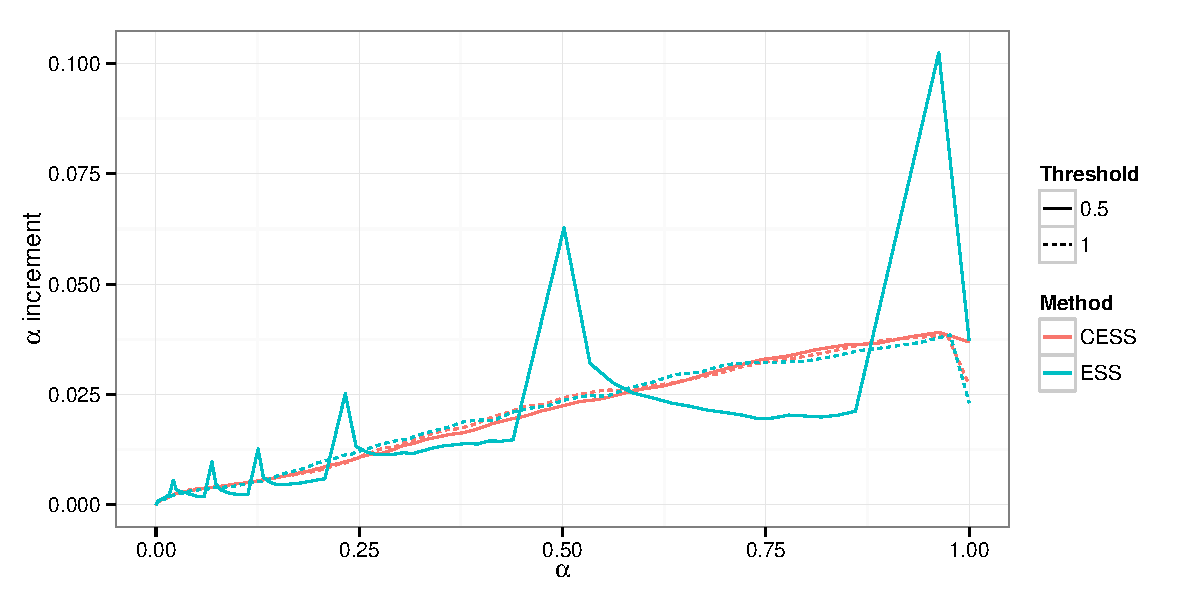
\includegraphics[width=\linewidth]{fig/Adaptive_Dist}
  \caption{A typical plot of $\alpha_t - \alpha_{t-1}$ against $\alpha_t$ (for
    the \pet compartmental model using \smc2 algorithm.) The specifications of
    the adaptive parameter (\ess or \cess) are adjusted such that all four
    samplers use roughly the same number of distributions.}
  \label{fig:adaptive_alpha}
\end{figure}

Figure~\ref{fig:adaptive_alpha} shows the variation of $\alpha_t -
\alpha_{t-1}$ with $\alpha_t$ when fixed reductions in \ess and \cess are used
to specify the sequence of distributions both when resampling is conducted
during every iteration (or equivalently, when the \ess falls below a threshold
of 1.0) and when resampling is conducted only when the \ess falls below a
threshold of 0.5. As is demonstrated in Section~\ref{sec:Illustrative
  Applications} the \cess-based scheme leads to a reduction in estimator
variance of around 20\% relative to a manually tuned (quadratic; see Section
\ref{sec:gmm_res}) schedule while the \ess-based strategy provides little improvement
over the linear case unless resampling is conducted during every iteration.

In addition to providing a significantly better performance at essentially no
cost, the use of the \cess emphasizes the purpose of the adaptive
specification of the sequence of distributions: to produce a sequence in which
the difference between each successive pair is the same (when using the \cess
one is seeking to ensure that the variance of the importance weights one would
arrive at if using $\pi_{t-1}$ as a proposal for $\pi_t$ is constant).

%% \ess only measures the performance of the particle system approximating the
%% target distributions, rather than the variances of the target distributions
%% themselves, which contributes to the variance of incremental weights. As seen
%% in equation~\eqref{eq:smc2-ds} and also for path sampling estimates when using
%% a geometric schedule, the variance of the incremental weights affect the
%% normalizing constants estimates directly. In the case of resampling at every
%% time step, the weights are directly normalized from the incremental weights.
%% In the general situation, as usual, let $W_{n-1}^{(i)}$ denote the
%% \emph{normalized weights} of particle $i$ at the end of time $t = n - 1$, and
%% $w_n^{(i)}$ denote the \emph{unnormalized} incremental weights of particle $i$
%% during the move at $t = n$. In the absence of resampling, we have the
%% recursive relationship,
%% \begin{equation*}
%%   W_n^{(i)} =
%%   \frac{W_{n-1}^{(i)}w_n^{(i)}}{\sum_{j=1}^NW_{n-1}^{(j)}w_n^{(j)}}
%% \end{equation*}
%% and the $\ess_n$,
%% \begin{equation}
%%   \ess_n = \frac
%%   {\bigl(\sum_{j=1}^NW_{n-1}^{(j)}w_n^{(j)}\bigr)^2}
%%   {\sum_{j=1}^N\bigl(W_{n-1}^{(j)}\bigr)^2\bigl(w_n^{(j)}\bigr)^2}
%% \end{equation}
%% If we do resampling after time $t = n - 1$ and before $t = n$, and let
%% $\bar{w}_n^{(i)}$ denote the new incremental weights after resampling, then we
%% have the new $\ess_n$, during move at $t = n$, as,
%% \begin{equation}
%%   \overline{\ess}_n = N \frac
%%   {\bigl(\sum_{j=1}^N\frac{1}{N}\bar{w}_n^{(j)}\bigr)^2}
%%   {\sum_{j=1}^N\frac{1}{N}\bigl(\bar{w}_n^{(j)}\bigr)^2}
%%   \label{eq:ess_before_res}
%% \end{equation}
%% \ess also provides information on ``smoothness'' of the sequence of
%% distributions in the sense that, it measures the discrepancy between sampling
%% distribution and the target distribution and if the target distributions
%% changes little, so shall be \ess. However, this link between \ess and the
%% ``smoothness'' is less direct. Another undesirable aspects of \ess is that its
%% evolution changes when different resampling strategies are used even when the
%% underlying target distributions are the same. Our motivation of extending the
%% concept of \ess is to adaptively place the distributions as if we do
%% resampling at every step without actually carrying out the resampling. Using
%% the unbiasedness of resampling, we can approximate $\overline{\ess}_n$ with
%% \begin{equation}
%%   \cess_n = \frac
%%   {\bigl(\sum_{j=1}^NW_{n-1}^{(j)}w_n^{(j)}\bigr)^2}
%%   {\sum_{j=1}^N\frac{1}{N}W_{n-1}^{(j)}\bigl(w_n^{(j)}\bigr)^2}
%% \end{equation}
%% where by $\cess_n$ we denote the ``conditional \ess'' as it depends upon a
%% consistent approximation of the variance of incremental weights. If we have
%% independent, identically distributed samples from the target distribution at
%% time $t = n - 1$, then $\cess_n$ tells us, essentially, how much variability
%% there would be in those incremental weights. And this variability reflects the
%% difference of the target distribution at time $t = n$ with the previous one.
%% This link is more obvious in the case where
%% equation~\eqref{eq:inc_weight_mcmc} is used to calculate the incremental
%% weights $w_n(x_{n-1},x_{n}$). Intuitively, \cess provides a direct measurement
%% of the ``smoothness'' of the sequence of distributions.

%% When resampling is performed at every step, then $\cess_n = \ess_n$.
%% Asymptotically, as the number of particles goes to infinity, adaptively
%% placing distributions such that $\cess_n = \cess^\star$ for a fixed value
%% $\cess^\star$ will give the same schedule as the resampling-every-time \ess
%% variant.

\subsection{Adaptive specification of proposals}
\label{sub:Adaptive specification of proposals}

The \smc sampler is remarkably robust to the mixing speed of \mcmc kernels
employed as can be seen in the empirical study below. However, as with any
sampling algorithms, faster mixing doesn't harm performance and in some cases
will considerably improve it. In the particular case of Metropolis-Hastings
kernels, the mixing speed relies on adequate proposal scales.

We adopt a simpler approach based on \cite{Jasra:2010eh}. They applied an idea
used within adaptive \mcmc methods \cite{Andrieu:2006tw}
to \smc samplers by using variance of parameters estimated from its particle
system approximation as the proposal scale for the next iteration, suitably
scaled with reference to the dimension of the parameters to be proposed.
Although, in practice we found that such an automatic approach does not always
lead to optimal acceptance rates it generally produces satisfactory results
and is simple to implement. In difficult problems alternative approaches to
adaptation could be employed; one approach demonstrated in
\cite{Jasra:2010eh} is to simply employ a pair of acceptance rate  thresholds
and to alter the proposal scale from the simply estimated value whenever the
acceptance rate falls outside those threshold values.

More sohisticated proposal strategies could undoubtedly improve performance
further and warrant further investigation. One possible approach is using the
Metropolis adjusted Langevin algorithm
(\mala; see \cite{Roberts:1996vd}). In summary, \mala derives a
Metropolis-Hastings proposal kernel for a target $\pi$ which satisfies
suitable differentiability and positivity conditions, from the Langevin
diffusion,
\begin{equation*}
  \diff L_t = \frac{1}{2}\nabla\log\pi(L_t)\diff t + \diff B_t
\end{equation*}
where $B_t$ is the standard Brownian motion. Given a state $X_{n-1}$, a new
state is proposed by discrete approximation to the above diffusion. That is,
for a fixed $h>0$,
\begin{equation}
  X_n\sim\calN\Bigl(X_{n-1}+\frac{1}{2}\nabla\log\pi(X_{n-1}), hI_d\Bigr)
\end{equation}
where $I_d$ is the identify matrix and $d$ is the dimension of the state
space. The new proposed state is accepted or rejected through the usual
Metropolis-Hastings algorithm. Compared to a ``vanilla'' random walk, which
often has very robust theoretical properties, \mala is attractive when it is
possible and its convergence conditions \cite{Roberts:1996vd} can be met,
because only one discrete approximation parameter $h$ needs to be tuned
for optimal performance. In addition, results from \cite{Roberts:2001ta}
suggested that \mala can be more efficient than a random walk when using
optimal scalings. We could also use the particle approximation at time index
$t = n - 1$ to estimate the covariance matrix of $\pi_{n}$ and thus tune the
scale $h$ on-line. As these algorithms are known to be somewhat sensitive to
scaling, and we seek approaches robust enough to employ with little user
intervention, we have not investigated this strategy here.

%A simpler alternative is based on the observation that in many situations,
%especially in Bayesian model comparison context (for example using a \smc2
%sampler for computing model evidences), the sampler starts with a distribution
%(e.g., the prior) whose parameters have large variances and moves towards a
%highly concentrated distribution (e.g., the posterior). Therefore it is
%sensible to have the proposal scales decays sequentially. One scheme to
%construct such a decay is having the proposal scale, say $\sigma$ decays in
%such a form $\sigma = \sigma^\star(b / (a + b\alpha))^p$ where $\sigma^\star$, $a$,
%$b$ and $p$ are constants controlling the speed of and end points of the decay
%and $\alpha$ is the schedule parameter which lies in $[0,1]$ (e.g., the
%$\alpha(t/T)$ in the previous geometric annealing scheme). The constants shall
%be chosen such that the accept rates of the random walk are controlled in an
%acceptable range for all distributions. Practically, one can afford using a
%relatively smaller number of particles and modest number of distributions as a
%pilot run of the algorithm. Using the pilot sampler to tune the constants.
%This simple alternative does indeed require some effort for choosing the
%constants. The benefit is one does not need to tune the proposal scales for
%many iterations, yet avoid the possible situation that with a fully automatic
%adaptation, the accept rates are not always satisfactory.
%
%In the special case of conjugate Normal prior, that is for data $\data$ and a
%parameter of interest $\mu$, $\data|\mu \sim \calN(\mu,\lambda^{-1})$ and
%$\mu \sim \calN(\xi, \kappa^{-1})$ and a geometric annealing scheme, namely
%$\pi_t(\mu)\propto\pi(\mu)[p(\data|\mu)]^{\alpha(t/T)}$, it is well known that
%at time $t$, $\pi_t(\mu)$ is a normal density with variance $(\kappa +
%n\lambda\alpha)^{-1}$ where $n$ is the number of data points. Therefore if we
%follow \cite{Jasra:2010eh} and use the parameter variance as proposal scale,
%the above scheme indeed produce the ``optimal'' scales with the constants
%properly chosen. In more general Bayesian modeling cases, with large amount of
%data, the posterior distribution are asymptotically Normal. This observation
%suggest more general usefulness of the above deterministic scheme.  Other
%specification of the decay is also possible. In section~\ref{sec:Illustrative
%  Applications} we demonstrate the effectiveness of this scheme empirically.
%
%Adaptive schemes for either a random walk or an \mala algorithm are
%conceptually appealing and require little computational cost and manual
%tuning. However in practice the results may not be satisfactory and the
%performance can depend on the type of the random walks. In contrast the
%deterministic automatic schemes give users more control of the tuning though
%the choice of the constants may not be obvious in interesting problems.

\section{An automatic, generic framework}
\label{sec:An automatic, generic framework}
